%%%%%%%%%%%%%%%%%%%%%%%%%%%%%%%%%%%%%%%%%%%%%%%%%%%%%%%%%%%%%%%%%%%%%%%%%%%
%%                                                                       %%
%%     LaTeX + CTeX 《数学杂志》论文模板, 只针对 A4 纸的中文Paper.       %%
%%                                                                       %%
%%                                                                       %%
%%                                                          2006.3.1     %%
%%     版本历史:                                                         %%
%%        Ver0.01   2005.09.10                                           %%
%%        Ver1.01   2006.03.01                                           %%
%%               1. 更改编号出现错位                                     %%
%%               2. 增加作者信息                                         %%
%%               3. 调整首页标题、作者和摘要之间的间距                   %%
%%     You can mofify it and distribute it freely                        %%
%%                                                                       %%
%%%%%%%%%%%%%%%%%%%%%%%%%%%%%%%%%%%%%%%%%%%%%%%%%%%%%%%%%%%%%%%%%%%%%%%%%%%

%%%%%%%%%%%%%%%%%%%%%%%%%%%%%%%%%%%%%%%%%%%%%%%%%%%%%%%%%%%%%%%%
%            中文稿 文章模板:A4 纸, 小五字, 单列              %
%%%%%%%%%%%%%%%%%%%%%%%%%%%%%%%%%%%%%%%%%%%%%%%%%%%%%%%%%%%%%%%%
\documentclass[a4paper,11pt,onecolumn,twoside]{ctexart}
\usepackage{amsmath,amssymb,amsfonts,amsthm,fancyhdr}
\usepackage{epsfig,graphicx,picins,picinpar,subfigure}
\usepackage{pstricks}
\usepackage{fancyvrb}
\usepackage[numbers,sort&compress]{natbib}
\headsep=0.5truecm \footskip 0pt \topmargin 0pt \oddsidemargin 0pt
\evensidemargin 0pt \setlength{\textwidth}{14.8truecm}
\setlength{\textheight}{21.5truecm}
\renewcommand{\theequation}{\arabic{section}.\arabic{equation}}
\setcounter{page}{1}
 \pagestyle{fancy} \fancyhf{}
\renewcommand{\headrulewidth}{0.4pt}

%%%%%%%%%%%%%%%%%%%%%%%%%%%%%%%%%%%%%%%%%%%%%%%%%%%%%%%%%%%%%%%%
%        文章正文                                              %
%%%%%%%%%%%%%%%%%%%%%%%%%%%%%%%%%%%%%%%%%%%%%%%%%%%%%%%%%%%%%%%%
\begin{document}

\CTEXoptions[figurename={Figure}] \CTEXoptions[tablename={Table}]
\CTEXoptions[bibname={\normalsize 参~~考~~文~~献}]

%%%%%%%%%%%%%%%%%%%%%%%%%%%%%%%%%%%%%%%%%%%%%%%%%%%%%%%%%%%%%%%%
%%-------------------- 作者提供的信息 ------------------------%%
%%%%%%%%%%%%%%%%%%%%%%%%%%%%%%%%%%%%%%%%%%%%%%%%%%%%%%%%%%%%%%%%
%\newcommand{\authors}{第一作者, 第二作者}  % 仅用于页眉, 与\author{}中的一致
%\newcommand{\mytitle}{论文题目}            % 仅用于页眉, 与\title{}中的一致

%%%%%%%%%%%%%%%%%%%%%%%%%%%%%%%%%%%%%%%%%%%%%%%%%%%%%%%%%%%%%%%%
%%------------- 标题, 作者, 通信地址定义 ---------------------%%
%%%%%%%%%%%%%%%%%%%%%%%%%%%%%%%%%%%%%%%%%%%%%%%%%%%%%%%%%%%%%%%%

\title{\Large\textbf{论文题目}
\footnotetext[1]{\zihao{-5}\textbf{收稿日期:} XXXX-XX-XX\quad
                \quad \quad \textbf{接收日期:} XXXX-XX-XX}
\footnotetext[0]{\zihao{-5}\textbf{基金项目:}XXXX基金资助~(12345678);
XXXX基金资助~(12345679).}
\footnotetext[0]{\zihao{-5}\textbf{作者简介:}
第一作者(出生时间--), 性别, 民族(汉族省写), 籍贯, 职称,
主要研究方向: xxxxxx. E-mail:xxxxx@xxxx.xxx.xx.}}




%%%%%%%%%%%%%%%%%%%%%%%%%%%%%%%%%%%%%%%%%%%%%%%%%%%%%%%%%%%%%%%%
% 作者姓名与单位 : 三种形式中选一种
% 后面英文摘要中的名字和单位同样处理
% ---------------------
% 第一种形式: 单一作者
% ---------------------
%\author{作者\\[-1pt]
%({\zihao{-5}作者单位(到部门),~~省市\, 邮政编码}) \\[-2pt]}

% ---------------------
% 第二种形式: 同一单位 多个作者 -- 名字左右并列,
% ---------------------
\author{\zihao{5}第一作者$^{1,2}$~, ~第二作者$^{2}$\\[-1pt]
({\zihao{-5}1.作者单位(到部门),~省~市~~邮政编码}) \\[-2pt]
({\zihao{-5}2.作者单位(到部门),~省~市~~ 邮政编码}) \\[-2pt]}



\date{}  % 这一行用来去掉默认的日期显示
\maketitle \vspace{-8mm}
%%%%%%%%%%%%%%%%%%%%%%%%%%%%%%%%%%%%%%%%%%%%%%%%%%%%%%%%%%%%%%%%
%  中文摘要
%%%%%%%%%%%%%%%%%%%%%%%%%%%%%%%%%%%%%%%%%%%%%%%%%%%%%%%%%%%%%%%%
\begin{center}
\begin{minipage}[c]{14cm}
\zihao{-5} \mbox{}\hspace{2.4em}{\CJKfamily{hei}摘~要:}\quad
本文研究了$\cdots\cdots$的问题. 利用$\cdots\cdots$的方法,
获得了$\cdots\cdots$结果,
推广了$\cdots\cdots$结果(即对结果的分析). \\
\mbox{}\hspace{2.4em}{\CJKfamily{hei}关\,键\,词:}\quad 关键词1; 关键词2; 关键词3; 关键词4\\
\mbox{}\hspace{2.4em}{\CJKfamily{hei}MR(2010)主题分类号:}\quad
XXXX ; XXXX \quad \quad \quad
\mbox{}\hspace{2.4em}{\CJKfamily{hei}中\,图\,分\,类\,号:}\quad
XXXX  \\
\mbox{}\hspace{2.4em}{\CJKfamily{hei}文\,献\,标\,识\,码: }\quad A
\quad \quad \quad
\mbox{}\hspace{2.4em}{\CJKfamily{hei}文\,章\,编\,号:}\quad 0255-7797(2007)07-0001-00\\

\end{minipage}
\end{center}

%%%%%%%%%%%%%%%%%%%%%%%%%%%%%%%%%%%%%%%%%%%%%%%%%%%%%%%%%%%%%%%%
%  正文由此开始
%%%%%%%%%%%%%%%%%%%%%%%%%%%%%%%%%%%%%%%%%%%%%%%%%%%%%%%%%%%%%%%%
\zihao{5}
%%%%%%%%%%%%%%%%%%%%%%%%%%%%%%%%%%%%%%%%%%%%%%%%%%%%%%%%%%%%%%%%
\vskip 0mm \noindent {\large {\bf 1 ~引言}} \vskip 3mm
\setcounter{section}{1}\setcounter{equation}{0}
%%%%%%%%%%%%%%%%%%%%%%%%%%%%%%%%%%%%%%%%%%%%%%%%%%%%%%%%%%%%%%%%


%%%%%%%%%%%%%%%%%%%%%%%%%%%%%%%%%%%%%%%%%%%%%%%%%%%%%%%%%%%%%%%%
\vskip 4mm \noindent {\large {\bf 2 ~新的一节}} \vskip 3mm
\setcounter{section}{2}\setcounter{equation}{0}
%%%%%%%%%%%%%%%%%%%%%%%%%%%%%%%%%%%%%%%%%%%%%%%%%%%%%%%%%%%%%%%%


这里给出了一些公式、表格、插图、引用等的例子, 仅供参考.
\begin{equation} \label{eq:1}
\left\{ \begin{aligned}
         \pi &= 3.141\cdots \\
     \sqrt{2}&=1.414\cdots
         \end{aligned} \right.
\end{equation}

\begin{eqnarray}
         \pi &=& 3.1415926\cdots \nonumber \\
             &\approx & 3.14.
\end{eqnarray}


$$\begin{aligned}
         \pi &= 3.1415926\cdots  \\
             &\approx  3.14.
\end{aligned}$$


$$\begin{aligned}
         \pi &= 3.1415926\cdots  \\
             &\approx  3.14.
\end{aligned}\eqno(2.3)$$



\begin{figure}[htbp]
\centering
\includegraphics[width=10cm,height=3cm]{figs/sin.eps}\\
\small{图1: 一个浮动图}
\end{figure}


\begin{figure}[htbp]
\begin{minipage}[t]{0.45\linewidth}
\centering
\includegraphics[width=6cm,height=3cm]{figs/sin.eps}\\
\small{图2: 这是第一个子图}
\end{minipage}%
\hfill
\begin{minipage}[t]{0.5\linewidth}
\centering
\includegraphics[width=5cm,height=3cm]{figs/fig.eps}\\
\small{图3:这是第二个子图}
\end{minipage}
\end{figure}




{\bf 定义~ 2.1}~$^{[1]}$~~~~    %这是定义内容.



{\bf 引理~ 2.2}~$^{[2]}$~~    %这是引理内容.




{\bf 定理~ 2.3~~}  %这是定理内容.




{\bf 证~~}     %这是定理的证明.



{\bf  推论~ 2.4~~}  %这是推论.



下面是一些引用的例子:


{\bf 例~ 1~~} 这里引用了第2页的公式(2.1), 从下面的表1可见.


\begin{center}
 {\small 表~1~~   $\gamma$ 按照规则~II 产生的数值结果}
 \vskip 2mm
\begin{tabular}{ccccc}
  \hline
  % after \\: \hline or \cline{col1-col2} \cline{col3-col4} ...
 CPU数量 &  迭代次数 & 目标函数值 &  $\gamma^*$ & 运行时间(秒) \\
 \hline
   10 &  3+57 &     680.6300660&       2.2564 & 1.22\\
   15 &   3+66 &    680.6300592&      0.8235 &  1.35\\
    20 &    3+65 &     680.6300594&      0.6421 & 1.38\\
  \hline
  \end{tabular}
%}
\end{center}


%%%%%%%%%%%%%%%%%%%%%%%%%%%%%%%%%%%%%%%%%%%%%%%%%%%%%%%%%%%%%%%%
\vskip 4mm \noindent {\large {\bf 3 ~ 新的一节}} \vskip 3mm
\setcounter{section}{3}\setcounter{equation}{0}

%%%%%%%%%%%%%%%%%%%%%%%%%%%%%%%%%%%%%%%%%%%%%%%%%%%%%%%%%%%%%%%%

{\bf 注~~}
 进一步学习和提高中英文\LaTeX 排版的水平、掌握一些特殊的技巧,
 可参考文献[1--5].

\vspace{4mm}
%%%%%%%%%%%%%%%%%%%%%%%%%%%%%%%%%%%%%%%%%%%%%%%%%%%%%%%%%%%%%%%%
%  参考文献
%%%%%%%%%%%%%%%%%%%%%%%%%%%%%%%%%%%%%%%%%%%%%%%%%%%%%%%%%%%%%%%%
\zihao{-5}
\begin{thebibliography}{99}
%\setlength{\parskip}{0pt}  %段落之间的竖直距离
\addtolength{\itemsep}{-0.8 em} % 缩小参考文献间的垂直间距
  \bibitem{1}  李国平, 陈银通, 刘怀悛. 一级线性齐次差分方程组的一般性质[J]. 数学杂志, 1981, 1(1): 1--12.
  \bibitem{2} 胡宏昌, 孙海燕.
  半参数回归模型小波估计的稳定地依分布收敛性[J].
  武汉大学学报(理学版), 2003, 49(5): 571--574.
  \bibitem{3}  王梓坤. 随机过程论(第二版)[M]. 北京: 科学出版社, 1965.
  \bibitem{4}  辛希孟. 信息技术与信息服务国际研讨会论文集:A集[C].北京: 中国社会科学出版社, 1994.
  \bibitem{5} 樊保强. 大规模排序问题的列生成算法研究[D]. 上海: 同济大学博士学位论文, 2006.
  \bibitem{6} 钟文发. 非线性规划在可燃毒物配置中的应用[A].
  赵玮.运筹学的理论与应用-中国运筹学会第五届大会论文集[C]. 西安: 电子科技大学出版社, 1996: 468--471.
  \bibitem{7} 王明亮. 关于中国学术期刊标准化数据库系统工程的进展[EB/OL].
  http//www.cajcd.edu.cn/pub/wml.txt/980810-2.html, 1998-08-16/1998-10-04.
  \bibitem{8} Dawande M, Geismar H  N, Hall N G. Supply chain
scheduling: distribution systems [J]. Operations Research, 2007,
47(5): 511--517.
  \bibitem{9} Feller W.  An introduction to probability theory and its applications (3rd ed.)[M]. New York: Wiley, 1969.


\end{thebibliography}




%%%%%%%%%%%%%%%%%%%%%%%%%%%%%%%%%%%%%%%%%%%%%%%%%%%%%%%%%%%%%%%%
%  英文摘要
%%%%%%%%%%%%%%%%%%%%%%%%%%%%%%%%%%%%%%%%%%%%%%%%%%%%%%%%%%%%%%%%
\vspace{6mm}
\hspace{-8mm}
\parbox{\textwidth}{
\begin{center}
\large{\textbf{ENGLISH TITLE }}\\
\vspace{8mm}
\zihao{5}{Author1$^{1,2}$~,~Author1$^{2}$~}\\[2pt]
(\textit{\zihao{-5} 1.First Author's Working Unit (Up to Department), Province Zip ~ Code,China}) \\[2pt]
(\textit{\zihao{-5} 2.First Author's Working Unit (Up to Department), Province Zip ~ Code,China}) \\[2pt]
\end{center}

\begin{center}
\begin{minipage}[c]{14cm}
\zihao{-5}
 \hspace{2em}\textbf{Abstract:}
Here is the abstract... ... .\\
\mbox{}\hspace{2.3em}\textbf{Keywords:}\quad Keyword 1; Keyword 2; Keyword 3; Keyword 4.\\
\mbox{}\hspace{2.3em}\textbf{2010 MR  Subject Classification:}\quad XXXX ; XXXX\\

\end{minipage}
\end{center}}

%%%%%%%%%%%%%%%%%%%%%%%%%%%%%%%%%%%%%%%%%%%%%%%%%%%%%%%%%%%%%%%%
%  文章结束
%%%%%%%%%%%%%%%%%%%%%%%%%%%%%%%%%%%%%%%%%%%%%%%%%%%%%%%%%%%%%%%%
\clearpage
\end{document}
